
\section{Analyse}
\label{Analyse}

\subsection{Routing Engine}
\label{Analyse:Routing Engine}

In den Rahmenbedingungen (Kapitel \ref{Einführung:Rahmenbedingungen, Umfeld, Definitionen, Abgrenzungen}) wurde festgehalten, für die Implementation der "`\acs{ÖV}-Güteklassen 2018"' PostGIS~\cite{postgis} und die Routing-Engine pgRouting~\cite{pgRouting} zu verwenden, soweit dies die Technologie erlaubt.
Nachfolgend soll kurz aufgezeigt werden, welche alternativen Technologien in Frage kommen und ob die technische Machbarkeit mit PostGIS/pgRouting gegeben ist.

Für die Wahl einer Routing-Engine gibt es drei grosse Open-Source Lösungen, die sich bewährt haben: OSRM~\cite{osrm}, GraphHopper~\cite{graphhopper} und pgRouting.
Für unsere Zwecke sind folgende Kriterien massgebend:

\begin{enumerate}
    \item Das Erstellen von Isochronen
    \item Die Integration von Höhendaten
\end{enumerate}

Für das Kriterium 1 bringen GraphHopper und pgRouting bereits eingebaute Funktionen mit, für OSRM gibt es ein experimentelles Tool von Mapbox~\cite{mapbox_osrm_isochrone}.

Für das zweite Kriterium, die Integration von Höhendaten, gibt es bei GraphHopper und OSRM eingeschränkte Möglichkeiten. GraphHopper bietet zwar an, das weltweit abdeckende Modell von \ac{SRTM} direkt einzubinden, dessen Genauigkeit ist mit 90 Metern aber deutlich tiefer als bei unserem swissALTI$^{3D}$-Modell~\cite{swissalti3d_swisstopo} mit 2--10 Metern. Die Integration eines eigenen Modells würde bei beiden Routing-Engines eine Anpassung der Implementierung benötigen.

Bei pgRouting bringt die Implementation selbst keine direkte Unterstützung von Höhendaten an, im Unterschied zu den anderen Varianten kann die Kosten-Funktion zur Berechnung von Wegzeiten aber einfach selbst angepasst werden.
Durch die Benutzung von PostgreSQL mit PostGIS bietet dieser Ansatz deutlich mehr Flexibilität.
Das Terrainmodell kann in einer separaten Datenbank effizient als Raster persistiert und für die Kostenberechnung der einzelnen Kanten abgerufen werden.

Da die Fahrplandaten ebenfalls in relationaler Form in einer PostgreSQL-Datenbank gehalten werden, wird auch die Integration dieser Daten mit dem Routing-Graphen erleichtert.

Abschliessend kann man sagen, dass die Kriterien mit pgRouting erfüllt werden und sich von den drei evaluierten Routing-Engines am besten für die Integration mit den restlichen Daten (Fahrplan- und Höhendaten) eignet.

\subsection{Evaluation Frontend-Framework}
\label{Analyse:Evaluation Frontend-Framework}

Wie in den Rahmenbedingungen (Kap. \ref{Einführung:Rahmenbedingungen, Umfeld, Definitionen, Abgrenzungen}) vorausgesetzt, stehen für die Technologie der Web-Applikation (Frontend) die Optionen React~\cite{react} oder Vue.js~\cite{vuejs} zur Auswahl.
Die Wahl viel auf diese zwei Frameworks, da sich beide momentan schnell verbreiten und zum Design von \ac{SPA} ausgelegt sind, was für unsere Zwecke zum Darstellen einer Karte gut geeignet ist.
Ein grösseres Framework wie Angular wäre dafür zu gross, weshalb die Evaluation auf diese zwei leichtgewichtigeren Varianten eingeschränkt wird.

Vue.js und React werden im Folgenden anhand mehrerer Kriterien verglichen.
Als Demonstration wird mit beiden Varianten eine identische kleine Web-Applikation entwickelt.
Diese besteht aus einer Web-Karte und einem kleinen Kontrollelement, um einen zusätzlichen Layer einzublenden.
Der Code ist unter~\cite{github:playground} zu finden.

Zum Schluss wird ein Fazit gezogen und entschieden, welches Framework für das Frontend eingesetzt wird.

\subsubsection{Funktionsumfang}
\label{Analyse Framework:Funktionsumfang}

Sowohl React als auch Vue.js bauen auf sehr ähnlichen Prinzipien auf.
Applikationen werden in einzelne Komponenten zerteilt und aufeinander aufgebaut.
In einer Komponente ist jeweils die Darstellung (Template) und die UI-Logik miteinander gekoppelt.
Komponenten halten intern Daten, die von einer anderen Komponente bedingt verändert werden können.

Ein Unterschied liegt in der Defintion von HTML-Templates.
Vue.js verwendet reines HTML mit einer erweiterten Template-Syntax, ähnlich wie bei herkömmlichen Template-Engines.
React dagegen benutzt JSX~\cite{jsx}, eine spezielle Syntax, bei der JavaScript und HTML gemischt werden können.
In einem Zwischenschritt wird dies zu JavaScript kompiliert, das schlussendlich HTML-Elemente erstellt.
Dies macht React etwas angenehmer, da in den Templates direkt beliebiges JavaScript eingebunden werden kann.
Bei Vue.js sind nur einzelne Expressions nötig, und der Rest der Syntax muss HTML-kompatibel sein.
So werden z.B. JavaScript-Variablen wie \code{myVar} in die HTML-kompatible Form \code{my-var} umgewandelt, was bei der Benutzung verwirrend sein kann.

React wird von Facebook entwickelt und ist etwas älter (2013) als Vue.js (2014), das unabhängig unterhalten wird.
Dadurch gibt es beim Paket-Repository von NPM mehr vorgefertigte Komponenten für React (ca. 50'000 verglichen mit ca. 10'500 für Vue.js).
Die Unterstützung und Wartung von Facebook spricht dafür, dass React auch in den nächsten Jahren stets weiter entwickelt wird.

Beide Frameworks sind aber schlank gehalten und bieten nur die Kernfunktionalitäten.
Erweiterte Komponenten wie Routing oder State-Management sind in andere Frameworks ausgelagert, welche jeweils eingebunden werden können.

Insgesamt haben React und Vue.js einen sehr ähnlichen Funktionsumfang und verwenden fast identische Prinzipien.

\subsubsection{Integration Leaflet}
\label{Analyse Framework:Integration Leaflet}

Für das Einfügen einer Web-Karte mit Raster-Kacheln in eine Web-Applikation hat sich die Library \emph{Leaflet}~\cite{leaflet} bewährt.
Es wird analysiert, wie fortgeschritten die Leaflet-Unterstützung in den jeweiligen Frameworks ist.

Für React bietet \emph{react-leaflet}~\cite{react-leaflet} die Funktionalität von Leaflet an, das Equivalent für Vue.js bildet \emph{Vue2Leaflet}~\cite{vue2leaflet}.

Beide Komponenten bieten eine rudimentäre Dokumentation an, die Bedienung wird aber erst mit den zahlreichen Beispielen klar.
Von der Funktionalität her ist kein grosser Unterschied festzustellen.
\emph{Vue2Leaflet} bildet zwar nicht die komplette Leaflet-Library ab, die für diese Arbeit benötigten Funktionen sind aber alle vorhanden.


\subsubsection{Integration Vector Tiles}
\label{Analyse Framework:Integration Vector Tiles}

Vector Tiles sind Kacheln, die Ausschnitte aus Karten als Vektoren darstellen, anstatt wie bei Raster-Kacheln mit simplen Bildern~\cite{geometalab_vectortiles}.
Dies hat unter anderem den Vorteil, dass nicht bei jeder Zoomstufe ein neues Bild geladen werden muss, sondern die Vektoren beliebig vergrössert werden können.

Für die Integration solcher Vector Tiles in Webkarten hat die Firma Mapbox ein Format spezifiziert und mit \emph{Mapbox GL JS} eine JavaScript-Library veröffentlicht, um diese einzubinden.~\cite{mapbox_gl_js}
Diese Library bietet deutlich mehr Möglichkeiten als Leaflet, die Darstellung von Kacheln individuell anzupassen.
Die Vektor-Daten selbst sind bei Mapbox bis zu einem gewissen Abrufvolumen kostenlos erhältlich.
Es können aber auch andere Datenquellen, wie z.B. von OpenMapTiles~\cite{openmaptiles}, verwendet werden.

Für die Integration mit React und Vue.js gibt es mehrere vorgefertigte Komponenten von Dritten.
Wir haben jeweils die beliebtesten (Anzahl Github-Stars) davon angeschaut.
Für React ist dies \emph{react-mapbox-gl}~\cite{react_mapbox_gl}, für Vue.js \emph{vue-mapbox-gl}~\cite{vue_mapbox_gl}.

Die React-Komponente ist gut dokumentiert und relativ einfach zu benutzen.
Die einzelnen Komponenten sind sauber in React-Komponenten abgebildet, was das Handling mit mehreren Layern angenehm macht.

Dagegen ist die Vue.js-Komponente nur ein einfacher Wrapper um die API von \emph{Mapbox GL}.
So kann z.B. ein zusätzlicher Layer nicht direkt im Template eingebunden werden, sondern muss über Event-Handling nach dem Laden der Karte hinzugefügt werden.
Dies macht das dynamische Hinzufügen und Entfernen von Karten-Elementen, was wir in unserer Applikation viel benötigen, sehr mühsam.

\subsubsection{Lernkurve}
\label{Analyse Framework:Lernkurve}

Die Lernkurve beschreibt under anderem, wie viel Zeit benötigt wird, sich in die neue Technologie einzuarbeiten.
Dies ist durchaus ein subjektives Kriterium und hängt von unserem bestehenden Erfahrung mit anderen Web-Frameworks ab.

Die beiden sehr ähnlichen Philosophien von React und Vue.js weichen in gewissen Punkten stark von uns vertrauten Praktiken ab, so etwa die inhärente Kopplung von Darstellung und Logik, die in anderen Modellen wie MVC (Model-View-Controller) aufgespalten wird.
Insofern benötigen beide Varianten eine gewisse Einarbeitungszeit, um sich mit diesen Konzepten vertraut zu machen.

Bei React kommt zusätzlich die neue Syntax JSX~\cite{jsx} dazu, die zwar etwas angenehmer zu lesen ist, aber in vielen kleinen Punkten von bereits Bekanntem abweicht.
So mussten z.B. HTML-Attribute wie \code{for} umbenannt werden, um nicht eine Namenskollision mit JavaScript zu verursachen.

Die Template-Syntax von Vue.js ist deutlich vertrauter, auch weil sie sehr dem Stil von anderen Template-Engines ähnelt.
Vue.js erlaubt auch einiges an "`Syntactic Sugar"' in den Templates.
So ist simples Data-Binding mit Event-Handling direkt im Template möglich, während bei React dies separat behandelt werden muss.

Aus dieser Einschätzung kann man sagen, dass die Lernkurve bei Vue.js etwas flacher als bei React ist.

\subsubsection{Tooling}
\label{Analyse Framework:Tooling}

Da sowohl React wie auch Vue.js auf NodeJS aufsetzen und den Paketmanager NPM benutzen, ist das Tooling sehr ähnlich.

Um eine neue Applikation zu erstellen, bietet React das Tool \emph{create-react-app}~\cite{create_react_app} an.
Beim Ausführen kann man angeben, welche zusätzlichen Libraries (z.B. für Unit-Testing) man verwenden möchte.
Während der Entwicklung kann ausserdem ein lokaler Server gestartet werden, der jeweils automatisch das Browser-Fenster neu ladet, wenn sich der Source-Code geändert hat.

Vue.js bietet mit \emph{vue-cli}~\cite{vue_cli} ein ähnliches Tool an.
Um eine neue Applikation aufzusetzen, kann zwischen verschiedenen Templates gewählt werden.
Es gibt verschiedene Templates für z.B. unterschiedliche Grössen der geplanten Applikation.
Während der Entwicklung bietet \emph{vue-cli} die praktisch identischen Möglichkeiten wie das Tool für React.

Insgesamt kann zwischen den beiden Varianten in Sachen Tooling praktisch keinen Unterschied festgestellt werden.


\subsubsection{Auswertung}
\label{Analyse Framework:Auswertung}

Für die Bewertung wird jedem Kriterium einen Wert von 1 bis 6 zugewiesen, wobei 6 die Bestnote ist.
Jedes Kriterium wird anhand der Relevanz und Wichtigkeit in unserem Projekt gewichtet.

\begin{table}[ht]
    \centering
    \begin{tabular}{r l p{3cm} l l}
        \toprule
        \textbf{ID} &
        \textbf{Kriterium} &
        \textbf{Relatives Gewicht (0-1)} &
        \textbf{Vue.js} &
        \textbf{React} \\
        \midrule
        1     & \nameref{Analyse Framework:Funktionsumfang}           & 0.2           & 5 / 1.0   & 5 / 1.0  \\
        2     & \nameref{Analyse Framework:Integration Leaflet}       & 0.1           & 5 / 0.5   & 4 / 0.4  \\
        3     & \nameref{Analyse Framework:Integration Vector Tiles}  & 0.3           & 2 / 0.6   & 5 / 1.5  \\
        4     & \nameref{Analyse Framework:Lernkurve}                 & 0.2           & 4 / 0.8   & 3 / 0.6  \\
        5     & \nameref{Analyse Framework:Tooling}                   & 0.2           & 5 / 1.0   & 5 / 1.0  \\
        \bottomrule
        \multicolumn{3}{l}{\textbf{Total}}                                            & \textbf{21 / 3.9}
                                                                                                & \textbf{22 / 4.5} \\
    \end{tabular}
    \caption{Resultat der Frontend-Framework-Evaluation}
    \label{table:Resultat der Frontend-Framework-Evaluation}
\end{table}

Wie in der Tabelle \ref{table:Resultat der Frontend-Framework-Evaluation} zu sehen ist, sind React und Vue.js vor der Gewichtung der Kriterien sehr ähnlich bewertet.
Das Kriterium \nameref{Analyse Framework:Integration Vector Tiles} sorgt für den Ausschlag zu Gunsten von React.
Dieses Kriterium haben wir stark gewichtet, da die Web-Karte die Hauptkomponente unserer Web-Applikation bildet und mit \emph{Mapbox GL JS} deutlich mehr Flexibilität als Leaflet anbietet.
In diesem Punkt bieten die vorhandenen Komponenten für Vue.js nicht die gewünschte Qualität.

\subsection{ÖV-Güteklassen 2018 Generator}
\label{Analyse:ÖV-Güteklassen 2018 Generator}

Der \nameref{container:generator} Container ist für die Berechnung der "`ÖV-Güẗeklassen 2018"' verantwortlich.
Umgesetzt wird diese Komponente als Python-Applikation.
Für die Kommunikation und Integration mit den Umsystemen sind einige Libraries nötig, die im Folgenden kurz diskutiert werden.

\subsubsection{Integration mit PostgreSQL}
\label{analyse_generator:Integration mit PostgreSQL}

Für die Integration der GTFS-Daten und der Routing-Engine für die Berechnung der \glspl{Isochrone} ist eine Integration mit PostgreSQL nötig.
Die Routing-Engine läuft auf pgRouting, eine Erweiterung von PostGIS, das wiederum eine Erweiterung von PostgreSQL ist.
Insofern braucht es für beide Integrationen lediglich eine Möglichkeit, mit PostgreSQL zu kommunizieren.

Dazu bietet sich bei Python die relativ neue Library \emph{records}~\cite{records} an.

Für unsere Zwecke braucht es nur simple SQL-Abfragen, da ein Grossteil der Logik mit \glspl{Stored Procedure} auf dem SQL-Server selbst umgesetzt wird.

\subsubsection{Umgang mit Geometrien}
\label{analyse_generator: Umgang mit Geometrien}

In der Business-Logik des Generators wird viel mit Geometrien gehandhabt, die schlussendlich zu den "`ÖV-Güteklassen 2018"' verabeitet werden.
Hierzu hat sich die Python-Library \emph{Shapely}~\cite{shapely} bewährt.
Diese unterstützt die \gls{GEOS}-Funktionen, die PostGIS ebenfalls implementiert.
Somit können mit den Geometrien die gleichen Berechnungen wie auf der Datenbank vorgenommen werden, was für eine reibungslose Integration spricht.

Ebenfalls können Geometrien mit \emph{Shapely} direkt in \gls{GeoJSON} exportiert werden.
Dies erlaubt eine einfache Serialisierung, um die berechneten Resultate an das \nameref{container:Backend} weiter zu geben.

\subsection{Web-Applikation}
\label{analyse:Web-Applikation}

Wie in Kapitel \ref{Analyse:Evaluation Frontend-Framework} evaluiert, wird für die Web-Applikation React~\cite{react} verwendet.
Für unsere Zwecke werden zusätzlich dazu Libraries benötigt, die im Folgenden kurz aufgezeigt werden.

\subsubsection{Webkarte}
\label{analyse_webapp:Webkarte}

% TODO: Je nachdem, ob wir Leaflet oder Mapbox GL einsetzen



\subsection{Design Frontend}
\label{analyse:Design Frontend}

Für das Frontend (Web-Applikation mit React) wird für das Design des User Interface ein Entwurf in Form von Wireframes erstellt.
Das Wireframe der Standard-Ansicht ist in Abbildung \ref{fig:wireframe_main} dargestellt.
Die restlichen Wireframes sind im Anhang \nameref{appendix:wireframes} abgebildet.

\begin{figure}[ht]
    \centering
    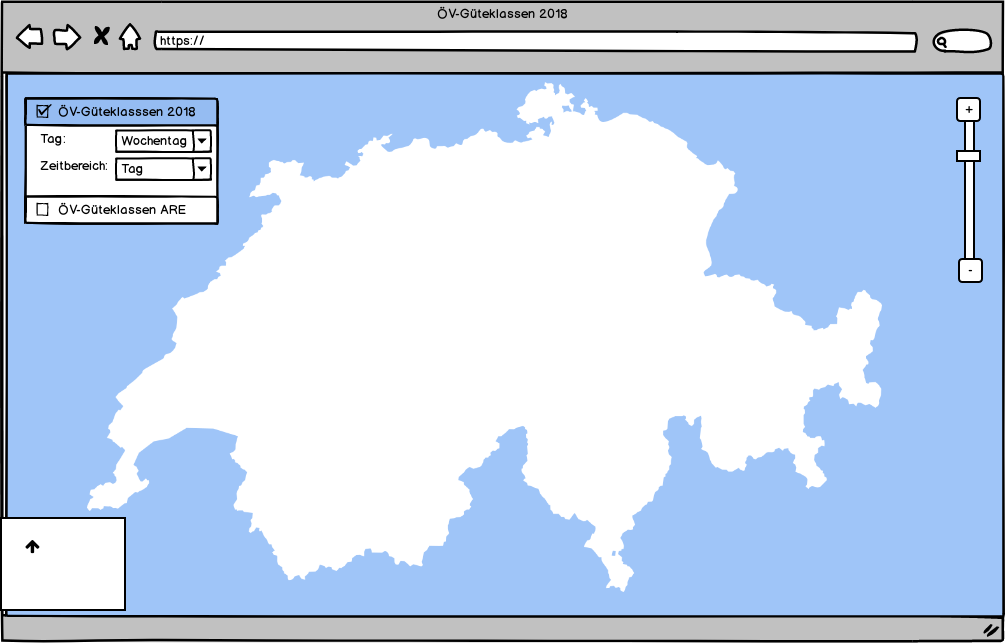
\includegraphics[width=1\linewidth]{projectdoc/img/wireframes/standardansicht.png}
    \caption[Wireframe der Standardansicht in der Web-Applikation]{Wireframe der Standardansicht in der Web-Applikation}
    \label{fig:wireframe_main}
\end{figure}

Grundsätzlich besteht das UI aus einer interaktiven Web-Karte, die sich über das gesamte Browser-Fenster erstreckt.
Darauf befindet sich ein Steuerelement, um die Anzeige der \glspl{ÖV-Güteklassen} zu konfigurieren.
Die beiden Karten-Layer der Datensätze \gls{OeVGK18} und \gls{OeVGK93} können ein- oder ausgeblendet werden.
Bei der \gls{OeVGK18} können zusätzlich Parameter wie der Tag (Wochentag oder Wochenende) sowie der Zeitbereich (Tag, Abend oder Nacht) konfiguriert werden.

\subsubsection{Einschränkungen}
\label{Analyse:Einschränkungen}

%TODO
